\documentclass{article}

\usepackage{algorithmic}
\usepackage{amsmath}
\usepackage{graphicx}
\usepackage{hyperref}
\usepackage{booktabs}
\usepackage{verbatim}

\begin{document}

\title{Parallel Histogram Calculation in CUDA}
\author{Geoffrey Ulman\\
        CS706}
\date{November 2012}
\maketitle

\section{Glimpse}\label{glimpse}

Glimpse (\url{http://metsci.github.com/glimpse/}) is a Java library for building 2D data visualization applications which take advantage of GPU hardware, allowing users to rapidly explore large data sets. For example, OpenGL Shader Language is used to dynamically adjust the color scale applied to a 2D heat map like Figure \ref{heatmap}. The underlying data for both the heat map and color scale are stored in OpenGL textures, which allows utilization of the GPU texture cache to speed data lookups.

\begin{figure}
\centering
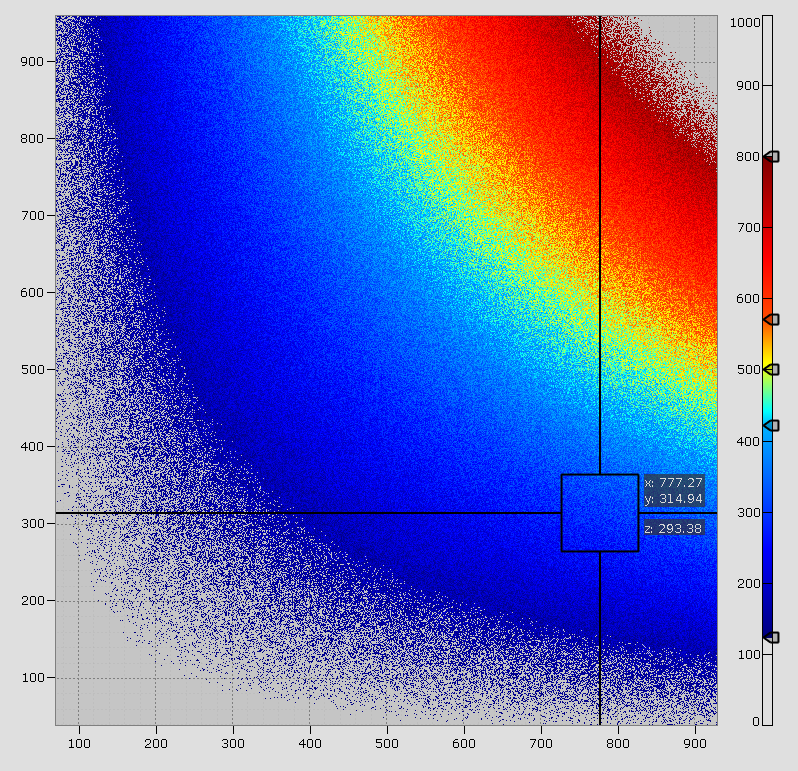
\includegraphics[width=0.9\textwidth]{TaggedHeatMapExample.png}
\caption{Glimpse Heat Map Visualization\\
         http://metsci.github.com/glimpse/screenshots.html}
\label{heatmap}
\end{figure}

\end{document}
